\documentclass[border=5pt]{standalone}
\usepackage{tikz}

\begin{document}
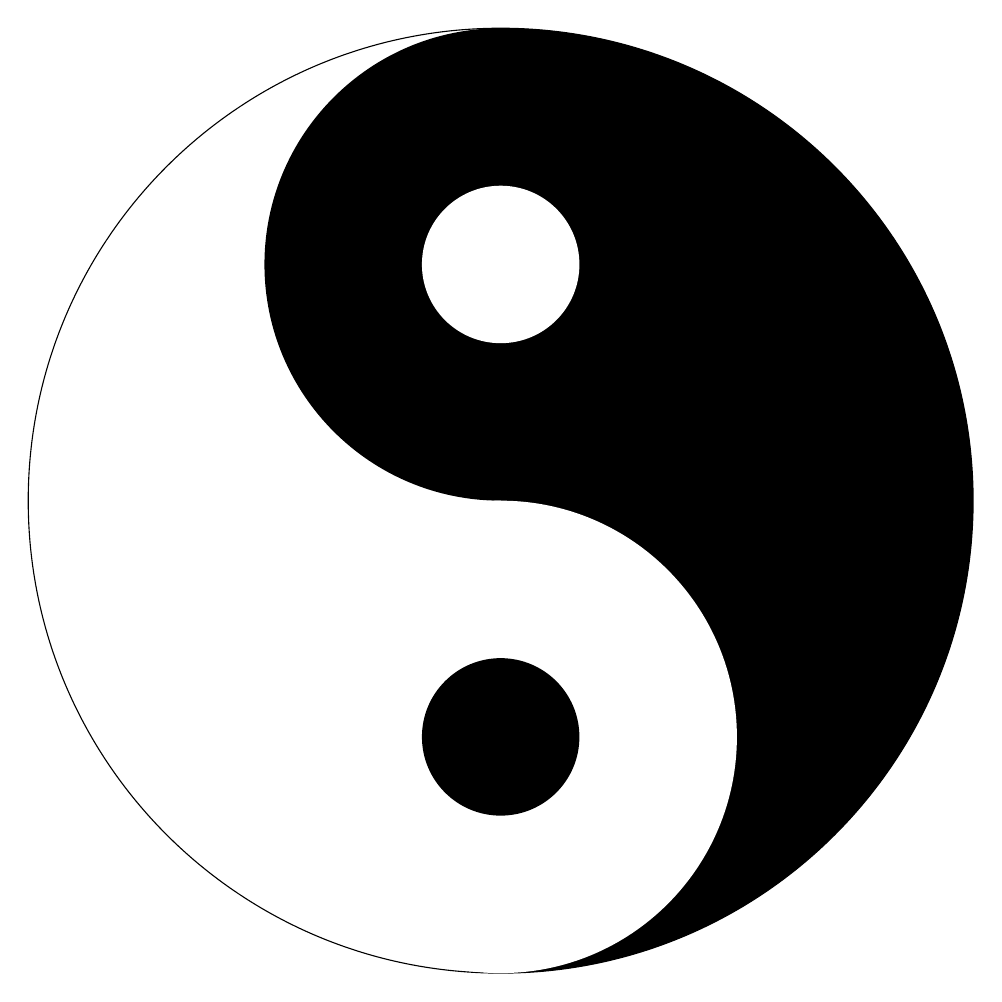
\begin{tikzpicture}

\def\R{6}
\draw[black] (0,0) circle(\R);  %画一个半径为\R的圆
%把圆的右半边填黑
\begin{scope}
  \clip(0,0) circle(\R);
  \fill[black] (0,-\R) rectangle (\R,\R);
\end{scope}

%把左边半圆的上面部分用大圆半径一半的中圆填黑
\fill[black] (0,\R/2) circle(\R/2);
%把左边半圆的上面部分用大圆半径一半的中圆填黑
\fill[white] (0,-\R/2) circle(\R/2);
%绘制上面的白色小圆:黑鱼的白眼
\fill[white] (0,\R/2) circle(\R/6);
%绘制下面的黑色小圆:白鱼的黑眼
\fill(0,-\R/2) circle(\R/6);

\end{tikzpicture}

\end{document}